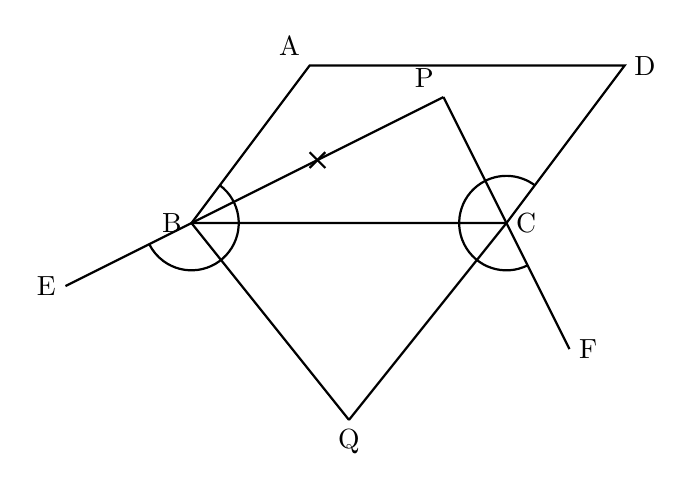
\begin{tikzpicture}[scale=1]

    % Define coordinates for the vertices of the parallelogram
    \coordinate (B) at (0, 0);
    \coordinate (C) at (4, 0);
    \coordinate (A) at (1.5, 2);
    \coordinate (D) at (5.5, 2);

    % Define coordinates for the intersection of interior bisectors P
    \coordinate (P) at (3.2, 1.6);
    
    % Q is shifted towards the bottom right from its previous position
    \coordinate (Q) at (2.0, -2.5);

    % Define extended points E and F so they form continuous straight lines with BP and PC
    % E is on the line extended backwards from P through B. 
    \coordinate (E) at (-1.6, -0.8);
    % F is on the line extended forwards from P through C. 
    \coordinate (F) at (4.8, -1.6);

    % Draw the edges of the parallelogram
    \draw[thick] (A) -- (B) -- (C) -- (D) -- cycle;

    % Draw the continuous straight lines for the bisectors and their extensions
    \draw[thick] (E) -- (P); % Straight line E-B-P
    \draw[thick] (P) -- (F); % Straight line P-C-F

    % Draw the lines meeting at Q
    \draw[thick] (B) -- (Q);
    \draw[thick] (C) -- (Q);

    % Draw the semi-circle arcs representing the bisected angles
    % Arc at B from line AB to line BE (sweeps clockwise from 53.13 to -153.43 degrees)
    \draw[thick] (0.36, 0.48) arc (53.13:-153.43:0.6);
    
    % Arc at C from line CF to line CD (sweeps clockwise through the interior side)
    % Angle of CF is -63.43 degrees (or 296.57 degrees). Angle of CD is 53.13 degrees.
    \draw[thick] (4.268, -0.537) arc (296.57:53.13:0.6);

    % Draw the tick mark (cross) on the segment BP exactly halfway
    \draw[thick] (1.5, 0.9) -- (1.7, 0.7);
    \draw[thick] (1.5, 0.7) -- (1.7, 0.9);

    % Add labels to all points exactly as positioned in the image
    \node[above left] at (A) {A};
    \node[left] at (B) {B};
    \node[right] at (C) {C};
    \node[right] at (D) {D};
    \node[above left] at (P) {P};
    \node[below] at (Q) {Q};
    \node[left] at (E) {E};
    \node[right] at (F) {F};

\end{tikzpicture}